\documentclass[conference]{IEEEtran}
\IEEEoverridecommandlockouts
% The preceding line is only needed to identify funding in the first footnote. If that is unneeded, please comment it out.
\usepackage{cite}
\usepackage{amsmath,amssymb,amsfonts}
\usepackage{algorithmic}
\usepackage{graphicx}
\usepackage{tabularray}
\usepackage{textcomp}
\usepackage{xcolor}
\def\BibTeX{{\rm B\kern-.05em{\sc i\kern-.025em b}\kern-.08em
    T\kern-.1667em\lower.7ex\hbox{E}\kern-.125emX}}
\begin{document}

\title{ME547MidtermReport}
\author{Tyler Allen Freitas}
\date{January 2024}

\title{ME547 Final Report: \\ Controlling a Vectored Thrust Aircraft}

\author{\IEEEauthorblockN{Tyler Freitas}
\IEEEauthorblockA{\textit{ME547 student} \\
\textit{University of Washington}\\
Seattle, WA, USA \\
tfreita@uw.edu}
}

\maketitle
\begin{abstract}
The following analysis models a 2D vectored thrust aircraft and simulates State-Feedback and Observer State-Feedback controllers with different thruster inputs. This nonlinear model is derived from Newton's laws of motion and linearized around its equilibrium points using Jacobian Linearization and small angle approximation. A simulation showed the aircraft's position was stable for these inputs (a step, an impulse, and a sine wave at different frequencies). The next step for this analysis will be implementing a nonlinear controller and simulating Vertical Takeoff and Landing (VTOL) maneuvers.
\end{abstract}

\section{Introduction}
The study of motion controls can be explored in many mechanical system applications. Motion controls have been implemented on aircraft for many years to control structural components including ailerons, elevators, and rudders. In recent decades, the Harrier jump jet has introduced the possibility of vertical takeoff and landing [1]. Specifically, the direction of the thrusters changes from a horizontal to a downward position [1]. To navigate these vertical maneuvers, a Linear Quadratic Regulator (LQR) [1] and a Nonlinear State-Feedback Controllers [2] are examples of controllers that are implemented for positional stability. This paper will focus on controlling a hovering vectored thrust aircraft with State-Feedback and Observer State-Feedback controllers.  

\section{Problem Formation}
\subsection{Model/Plant}
This system's model (plant) is a vectored thrust aircraft, which is analyzed as a rigid body in 2D space. This model has 3 thrusters: 1 thruster passing through the aircraft centroid, and 2 angled thrusters near the wingtips [1]. Note that these wingtip thrusters are used for aircraft stability [1]. These 3 thrusters are coupled together and move as a unit. Therefore, the changes in the wingtip thruster angles are the same. Fig. 1 displays the free body diagram  (FBD) of the plant.  This diagram is in the Cartesian Coordinates System. The system outputs are the aircraft position ($x$, $y$) and orientation ($\theta$). Note that the simulation outputs are only the horizontal ($x$) and vertical ($y$) positions. The reaction forces of the thrusters are translated to a common intersection point, and $r$ is the distance from this common intersection point of the thrusters to the aircraft centroid [1]. Additionally, these reaction forces are combined and broken down into horizontal ($F_1$) \& vertical ($F_2$) components which are the inputs for this plant. The other arrows in this FBD are the applied thruster forces. Note that this FBD neglects air drag forces.

\subsection{Free-Body Diagram}
\begin{figure}[!htbp]
\centerline{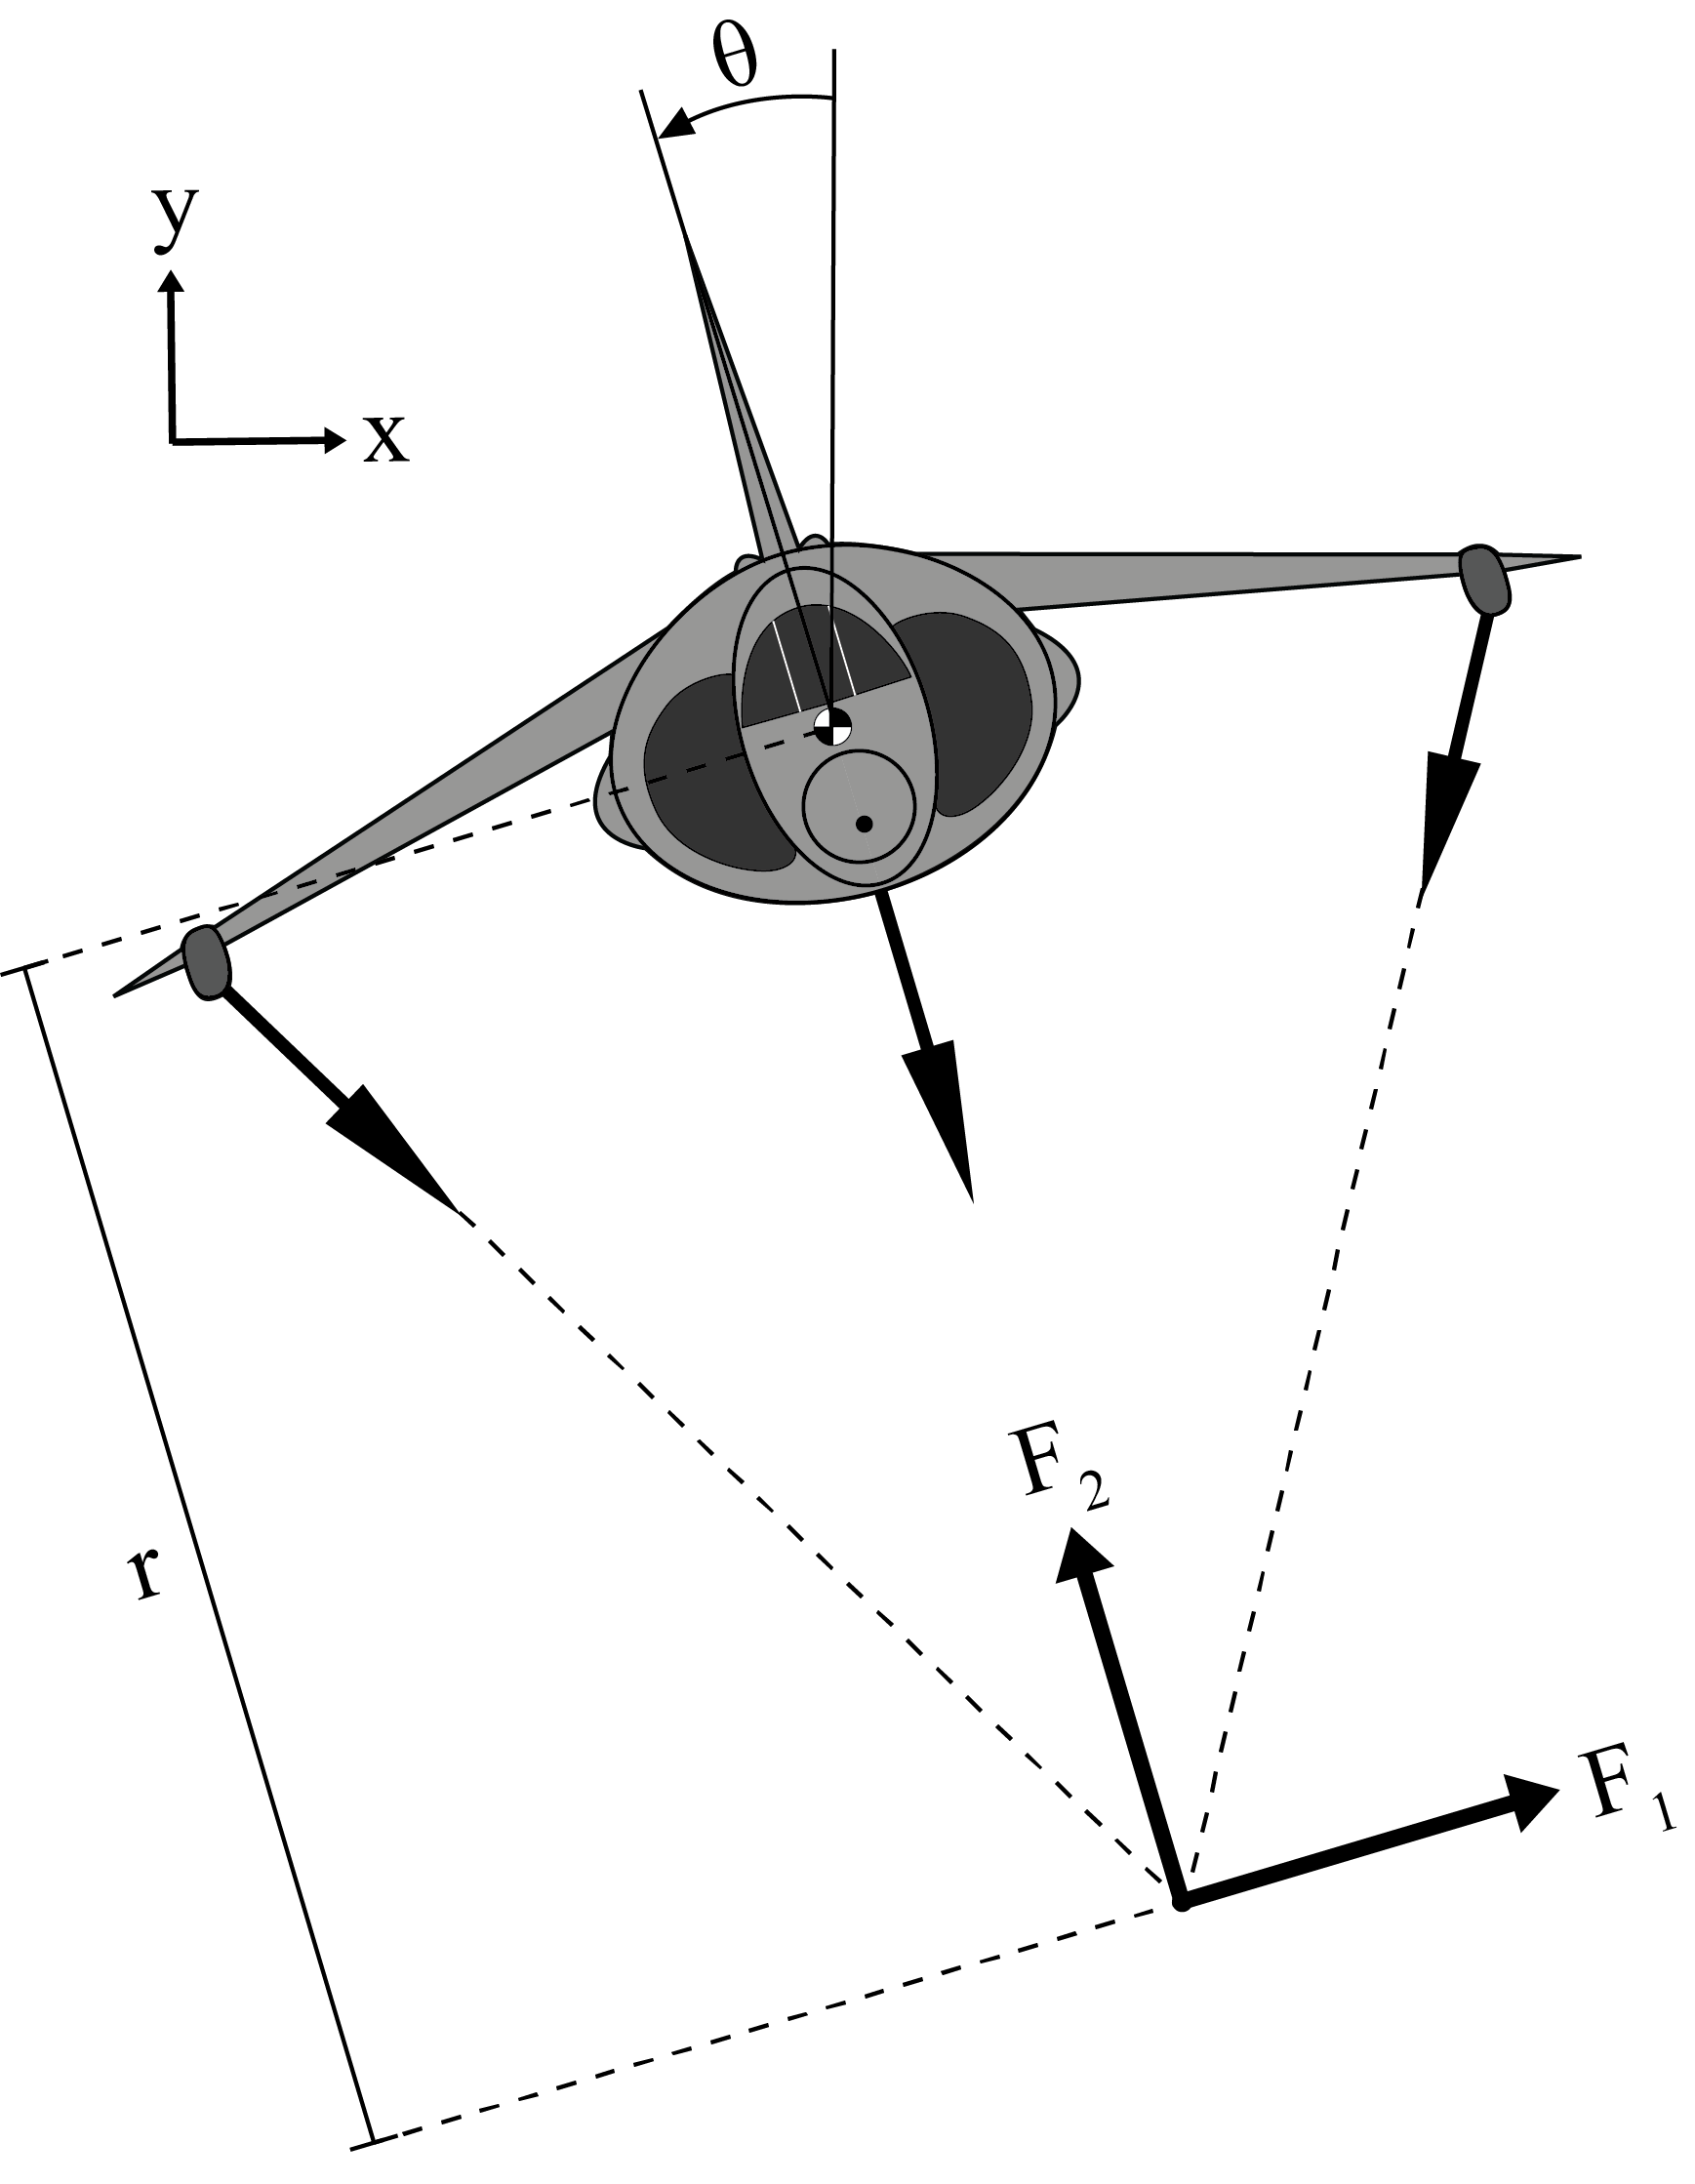
\includegraphics[scale = 0.3]{547_Midterm_FBD_bkg.png}}
\caption{2D Vectored Thrust Aircraft Free Body Diagram}
Note: This diagram is not to scale.
\label{figure1}
\end{figure}

\subsection{Physics:}
The aircraft can be represented as an airfoil that experiences aerodynamic forces (lift \& drag) from the air pressure distribution and shear stresses. The lift force counteracts the weight of the aircraft, and the thrust reduces the drag. Based on Newton’s $3^{rd}$ law, the applied downward thruster forces will have equal and opposite reactions, which are the aircraft lift forces. Also, the differential pressures across the aircraft area will create lift. The weight of the system is the aircraft mass. Drag is created by air and the vertical thruster reactions in the drag direction. The air stream leaving the thrusters is a laminar flow because the vertical maneuvers are at low speeds. The translational air drag, which opposes the direction of motion, is equal to the velocity times the damping coefficient ($c$) 
 ($F_{drag} = cx^\prime$). Note that the $1^{st}$ derivative of the aircraft position is velocity. $c$ depends on the frictional forces from the shear stresses along the aircraft surface and the air pressure distribution in the drag direction.\\

Newton's $2^{nd}$ law of motion is valid for this dynamic model because the aircraft's position and orientation change in time. This law states the summation of forces equals the mass times acceleration. Similarly, the summation of torques equals the moment of inertia times angular acceleration. Note that the $2^{nd}$ derivative of position is the aircraft acceleration. Based on the FBD in Fig. 1, the system forces are air drag, reaction forces by the thrusters, and weight. These forces are broken down into their respective x and y components (Equations 1 \& 2). Note that these model equations apply to a hovering aircraft with no external disturbances. For Equation 3, the only torque on the aircraft is from the thruster reaction ($F_1$). Note that there is no air torque resistance in Equation 3.

\subsection{Nonlinear Differential Equations [1]:} 
\[
mx^{\prime\prime} = F_1cos\theta - F_2sin\theta - cx^{\prime}  \tag{1}
\] 
\[
my^{\prime\prime} = F_1sin \theta + F_2cos\theta - mg - cy^\prime \tag{2}
\]
\[
J\theta^{\prime\prime} = rF_1 \tag{3} 
\]\\
Fig. 2 shows a nonlinear block diagram in Simulink. \\
Note: u1 = $F_1$ and u2 = $F_2-mg$ are dummy variables in this block diagram. \\
\vspace{-1.25mm}
\begin{figure}[!h]
\centerline{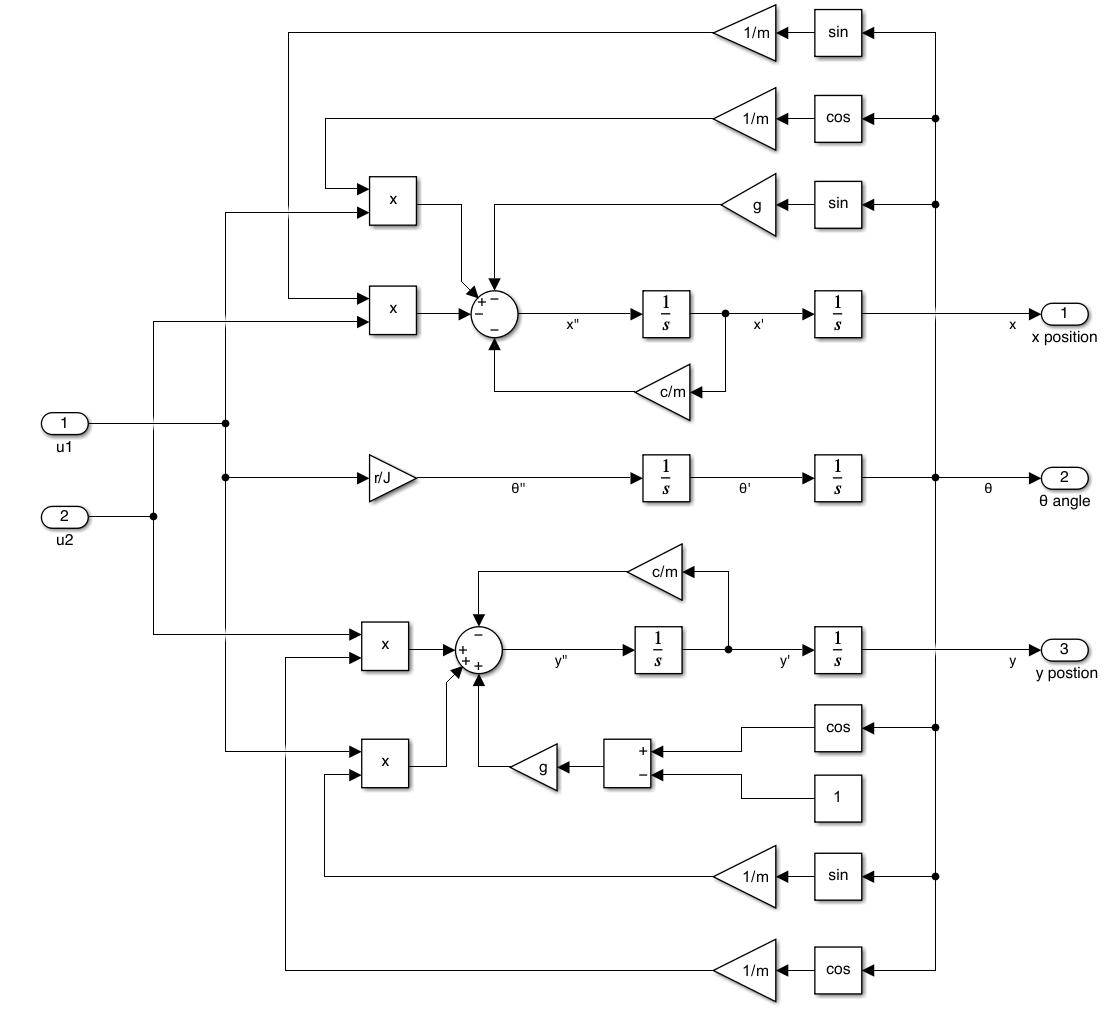
\includegraphics[scale=0.25]{non-linear_Block_Diagram.png}}
\caption{Nonlinear Block Diagram}
\label{figure}
\end{figure}

\subsection{Nonlinear Differential Equation Observations:}
This model has three coupled $2^{nd}$ order, ordinary differential equations. Note that these nonlinear equations have trigonometric functions. This system of equations is a continuous time model and a time-varying system because the response and the differential equation coefficients depend on time. The model is causal because the equations depend on the current states. As previously mentioned, this is a dynamic system as the aircraft's position and orientation change with respect to time. Table I lists the mathematical variables used in this analysis.\\

\begin{table}[htbp]
\begin{center}
\caption{Mathematical Variables}
\begin{tabular}{|p{2.9cm}|p{4.25cm}|c|}
\hline
\textbf{\textit{Variables}}& \textbf{\textit{Variable Name}}& \textbf{\textit{Units}} \\
\hline
$x$ & aircraft horizontal position & $m$\\
\hline
$x'$ & aircraft horizontal velocity & $m/s$\\
\hline
$x''$ & aircraft horizontal acceleration & $m/s^2$ \\
\hline
$y$ & aircraft vertical position & $m$ \\
\hline
$y'$ & aircraft vertical velocity & $m/s$ \\
\hline
$y''$ & aircraft vertical acceleration & $m/s^2$\\
\hline
$\theta$ & aircraft angular position & $rad$ \\
\hline
$\theta'$ & aircraft angular velocity & $rad/s$ \\
\hline
$\theta''$ & aircraft  angular acceleration & $rad/s^2$\\
\hline
$J$ & moment of inertia & $kg*m^2$ \\
\hline
$r$ & length from aircraft centroid to thrusters' intersection& $m$\\
\hline
$c$ & damping coefficient & $Ns/m$ \\
\hline
$g$ & acceleration due to gravity  & $m/s^2$ \\
\hline
$m$ & aircraft mass & $kg$ \\
\hline
$F_1$ & aircraft horizontal reaction & $N$ \\
\hline
$F_2$ & aircraft vertical reaction & $N$ \\
\hline
$y_e$ & y equilibrium point & $m$ \\
\hline
$x_e$ & x equilibrium point & $m$ \\
\hline
$z_e$ & state-space equilibrium points & $-$ \\
\hline
$F_e$ & input equilibrium points & $N$ \\
\hline
$A,B,C,D$ & state-space matrices & $-$ \\
\hline
$\zeta$ & linearized state-space variable & $-$\\
\hline
$v$ & linearized state-space input & $-$\\
\hline
$R$ & linearized state-space output & $-$\\
\hline
$z$ & nonlinear state-space variable & $-$\\
\hline
$f$ & time derivative of z & $-$\\
\hline
$h$ & nonlinear state-space output & $-$\\
\hline
$F$ & nonlinear state-space input & $-$.\\
\hline
$G_1$ & Local x transfer function & $-$\\
\hline
$G_2$ & Local y transfer function & $-$\\
\hline
$I$ & Identity Matrix &$-$ \\
\hline
$u$ & eigenvectors & $-$\\
\hline
$\lambda$ & eigenvalues & $-$\\
\hline
$J_A,J_B,J_C,J_D$ & Jordan Form state-space matrices  & $-$ \\
\hline
$V_g$ & Generalized Eigenvectors matrix & $-$ \\
\hline
$\beta$ & Similar Transform Variable & $-$ \\
\hline
$\Delta t$ & Sampling time & $s$ \\
\hline
$Q$ & Positive Definite Identity matrix & $-$ \\
\hline
$P$ & Lyapunov Symmetric Matrix & $-$ \\
\hline
$V$ & Lyapunov Function & $-$ \\
\hline
$K$ & State-Feedback Controller Parameter & $-$ \\
\hline
$L$ & Observer Controller Parameter & $-$ \\
\hline
$A_{obs},B_{obs},C_{obs},D_{obs}$ & Observable Canonical matrices  & $-$ \\
\hline
$A_d,B_d,C_d,D_d$ & Discrete state-space matrices  & $-$ \\
\hline
$A_{ctrl},B_{ctrl},C_{ctrl},D_{ctrl}$ & Controllable Canonical matrices  & $-$ \\
\hline
$K_{obs}$ & Observer State-Feedback Parameter & $-$ \\
\hline
$\omega$ & Sampling frequency & $rad/s$\\ 
\hline
$\hat{\zeta}$ & Observer State-Space Variable & $-$\\ 
\hline
\end{tabular}
\end{center}
\vspace{-5mm}
\end{table}

\section{Analysis}
This model is a system of nonlinear differential equations. Therefore, the system will be linearized around its equilibrium points with the Jacobian Linearization method [1]. These $2^{nd}$ differential equations are converted to a nonlinear state-space system, which is a system of $1^{st}$  order differential equations. $z$ is the nonlinear state-space variable for the state equation: ($z$ = ($z_1 = x$, $z_2 = y$, $z_3 = \theta$, $z_4 = x^\prime$, $z_5 = y^\prime$, $z_6 = \theta^\prime$)), and $F$ is the nonlinear input variable: ($F$ = ($F_1, F_2$)).\\
\newpage
Note: assume a small angle approximation around the equilibrium points: $sin(\theta) \approx \theta$ \& $cos(\theta) \approx 1$. The range of $\theta$ is from 0 to $2\pi$. Equations 4 and 5 show the nonlinear state-space and output equations respectively [1]. $f$ is the time derivative of $z$, and $h$ is the nonlinear state-space output.

\[
f(z,F) = \frac{dz}{dt} =
\begin{pmatrix}
z_4\\
z_5\\
z_6 \\
-\frac{c}{m}z_4 + \frac{F_1}{m} -\frac{F_2z_3}{m}\\
-g - \frac{c}{m}z_5 + \frac{F_1z_3}{m} +\frac{F_2}{m}\\
\frac{r}{J}F_1\\
\end{pmatrix}  
\tag{4}
\]

\[
h = 
\begin{pmatrix}
z_1\\
z_2\\
\end{pmatrix}
\tag{5}
\]
\subsection{Finding the Equilibrium Points:}
The equilibrium points are determined by setting these nonlinear system of equations (Equations 4 \& 5) to zero and solving for each $z$ and $F$ variable. \\

\noindent Stable Equilibrium Points: \\
\indent $z_e$ = ($z_1 = x_e$, $z_2 = y_e$, $z_3 = 0$, $z_4 = 0$, $z_5 = 0$, $z_6 = 0$)\\
\indent $F_e$ = ($F_1 = 0$, $F_2 = mg$)\\
Note: the system of equations above is independent of $x$ and $y$. \\

At a given equilibrium point ($x_e$ \& $y_e$), there is no rotational or translational velocity, and the horizontal reaction force ($F_1$) and $\theta$ are zero. The vertical reaction force ($F_2$) supports its weight. 

\subsection{Jacobian Matrices:}
Equations 6 and 7 compute the Jacobian Matrices for this nonlinear system [1].
\[ 
A = \frac{\partial f}{\partial z}\bigg|_{(z_e,F_e)}
B = \frac{\partial f}{\partial F}\bigg|_{(z_e,F_e)}
\tag{6}
\]
\[ 
C = \frac{\partial h}{\partial z}\bigg|_{(z_e,F_e)}
D = \frac{\partial h}{\partial F}\bigg|_{(z_e,F_e)}
\tag{7}
\]

The following 8-11 equations break down the Jacobian Matrices into the partial derivatives of $f$ and $h$ with respect to the nonlinear state-space variable ($z$) and nonlinear state-space input ($F$).
\vspace{-2mm}
\[
A = 
\begin{bmatrix}
\frac{\partial f_1}{\partial z_1}&\frac{\partial f_1}{\partial z_2}& \frac{\partial f_1}{\partial z_3}& \frac{\partial f_1}{\partial z_4}& \frac{\partial f_1}{\partial z_5} &\frac{\partial f_1}{\partial z_6}\\\\
\frac{\partial f_2}{\partial z_1}&\frac{\partial f_2}{\partial z_2}& \frac{\partial f_2}{\partial z_3}& \frac{\partial f_2}{\partial z_4}& \frac{\partial f_2}{\partial z_5} &\frac{\partial f_2}{\partial z_6}\\\\
\frac{\partial f_3}{\partial z_1}&\frac{\partial f_3}{\partial z_2}& \frac{\partial f_3}{\partial z_3}& \frac{\partial f_3}{\partial z_4}& \frac{\partial f_3}{\partial z_5} &\frac{\partial f_3}{\partial z_6}\\\\
\frac{\partial f_4}{\partial z_1}&\frac{\partial f_4}{\partial z_2}& \frac{\partial f_4}{\partial z_3}& \frac{\partial f_4}{\partial z_4}& \frac{\partial f_4}{\partial z_5} &\frac{\partial f_4}{\partial z_6}\\\\
\frac{\partial f_5}{\partial z_1}&\frac{\partial f_5}{\partial z_2}& \frac{\partial f_5}{\partial z_3}& \frac{\partial f_5}{\partial z_4}& \frac{\partial f_5}{\partial z_5} &\frac{\partial f_5}{\partial z_6}\\\\
\frac{\partial f_6}{\partial z_1}&\frac{\partial f_6}{\partial z_2}& \frac{\partial f_6}{\partial z_3}& \frac{\partial f_6}{\partial z_4}& \frac{\partial f_6}{\partial z_5} &\frac{\partial f_6}{\partial z_6}
\end{bmatrix}
\Bigg|_{(z_e,F_e)} 
\tag{8}
\] 

\[
\vspace{-2mm}
B = 
\begin{bmatrix}
\frac{\partial f_1}{\partial F_1}&\frac{\partial f_1}{\partial F_2} \\\\
\frac{\partial f_2}{\partial F_1}&\frac{\partial f_2}{\partial F_2} \\\\
\frac{\partial f_3}{\partial F_1}&\frac{\partial f_3}{\partial F_2} \\\\
\frac{\partial f_4}{\partial F_1}&\frac{\partial f_4}{\partial F_2} \\\\
\frac{\partial f_5}{\partial F_1}&\frac{\partial f_5}{\partial F_2}\\\\
\frac{\partial f_6}{\partial F_1}&\frac{\partial f_6}{\partial F_2}
\end{bmatrix}
\Bigg|_{(z_e,F_e)} 
\tag{9}
\] 

\[
C = 
\begin{bmatrix}
\frac{\partial h_1}{\partial z_1}&\frac{\partial h_1}{\partial z_2}& \frac{\partial h_1}{\partial z_3}& \frac{\partial h_1}{\partial z_4}& \frac{\partial h_1}{\partial z_5} &\frac{\partial h_1}{\partial z_6}\\\\
\frac{\partial h_2}{\partial z_1}&\frac{\partial h_2}{\partial z_2}& \frac{\partial h_2}{\partial z_3}& \frac{\partial h_2}{\partial z_4}& \frac{\partial h_2}{\partial z_5} &\frac{\partial h_2}{\partial z_6}
\end{bmatrix}
\Bigg|_{(z_e,F_e)} 
\tag{10}
\] 
\[
D =
\begin{bmatrix}
\frac{\partial h_1}{\partial F_1}&\frac{\partial h_1}{\partial F_2} \\\\
\frac{\partial h_2}{\partial F_1}&\frac{\partial h_2}{\partial F_2}
\end{bmatrix}
\Bigg|_{(z_e,F_e)} 
\tag{11}
\] 

\subsection{Linearized State-Space Equations \& Block Diagram:}
These Jacobian Matrices (Equations 14-17) create a linearized state-space system, which analyzes the local behavior around the equilibrium points [1]. New variables are created by subtracting the nonlinear state-space variable and input with its equilibrium points. Thus, $\zeta = z - z_e$\, which is the linearized state-space variable, $v = F - F_e$, which is the linearized state-space input variable, and R is the linearized state-space output variable. Equations 12 and 13 show the linearized state-space and output equations respectively [1].

\[
\zeta^\prime = A\zeta + Bv
\tag{12}
\] 
\[
R = C\zeta + Dv
\tag{13}
\] 

\[
A = 
\begin{bmatrix}
0&0& 0& 1& 0 &0\\
0 &0 &0 &0 &1 &0\\
0 &0 &0 &0 &0 &1\\
0 &0 &-g& -c/m &0 &0\\
0 &0 &0 &0 &-c/m &0\\
0 &0 &0 &0 &0 &0\\
\end{bmatrix}
\tag{14}
\]
\[
B = 
\begin{bmatrix}
0 &0\\
0 &0\\
0 &0\\
1/m& 0\\
0 &1/m\\
r/J& 0\\
\end{bmatrix}
\tag{15}
\] 

\[
C = 
\begin{bmatrix}
1&0&0&0&0&0\\
0&1&0&0&0&0\\
\end{bmatrix}
\tag{16}
\]
\[
D =
\begin{bmatrix}
0&0\\
0&0\\
\end{bmatrix}
\tag{17}
\] 

Fig. 3 displays a linearized block diagram in Simulink. \\
Note: The dummy variables, u1 \& u2, represent $F_1$ \& $F_2$ respectively in this block diagram. \\

\begin{figure}[htbp!]
\centerline{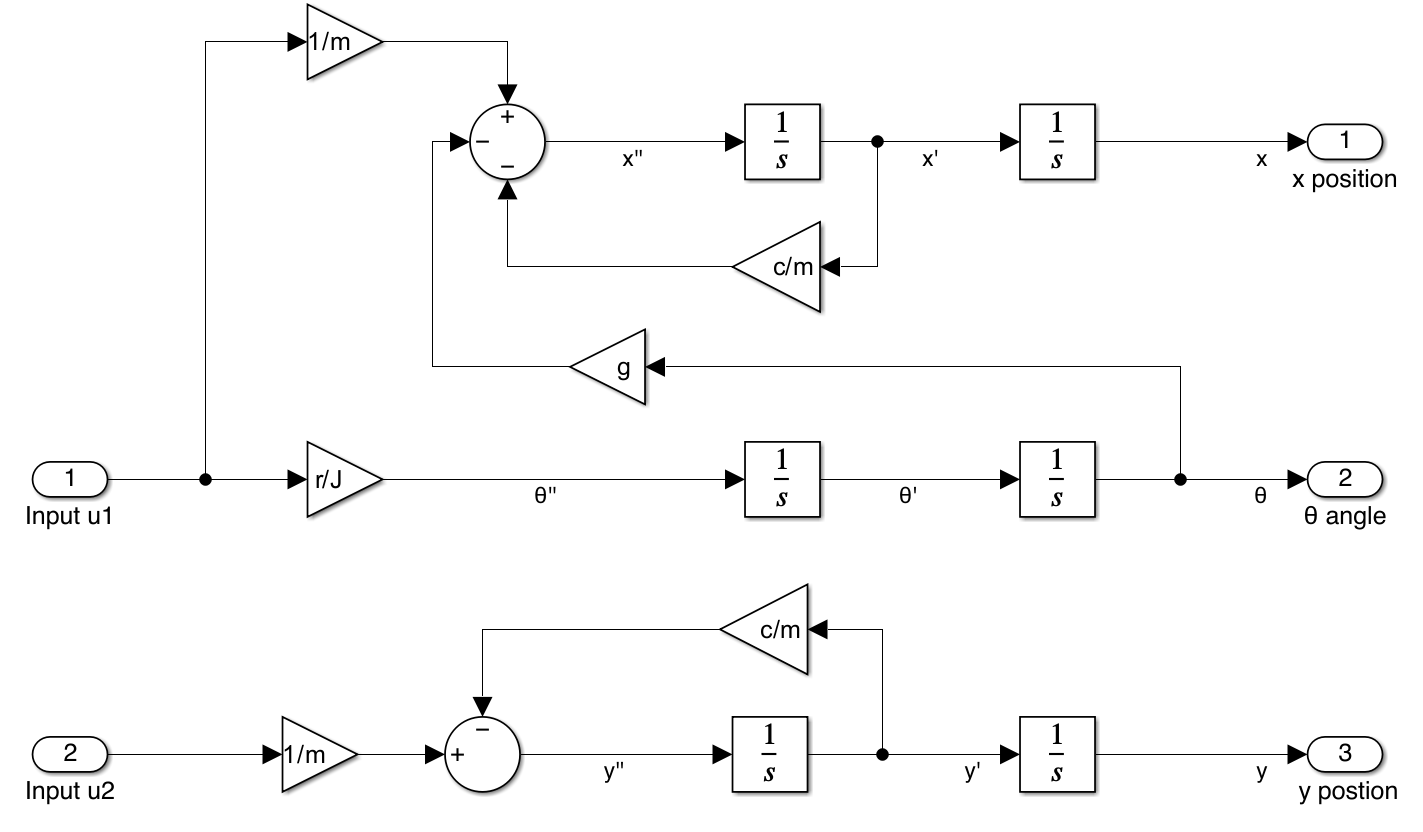
\includegraphics[scale=0.25]{LinearBlock.png}}
\caption{Linearized Block Diagram}
\label{figure}
\end{figure}



\subsection{Eigenvalue Stability Analysis}
The eigenvalues/poles of the A matrix determine the system stability. The system is stable if all of the real parts of the eigenvalues are negative. If the eigenvalues are on the imaginary axis in the complex plane, then the system is marginally stable. If a system has 1 positive real part pole, then the system is unstable. \\

 MATLAB uses the eigenvalues equation (Equation 18) to solve for the eigenvectors \& eigenvalues. The roots of the characteristic equation (Equation 19) are the eigenvalues of A.
 \[
(A - I\lambda)u = 0 \tag{18}
\]
\[
det(A - I\lambda) = 0 \tag{19}
\]
Eigenvalues of A are $\lambda =$ 0,0,0,0, -0.0125, \& -0.0125.\\
There are multiple eigenvalues at the origin, therefore this system is not asymptotically stable. \\

Note: the following model parameters (Table II) are used for numerical analysis \& simulation:\\
\begin{table}[h]

\begin{center}
\caption{Numerical Analysis \& Simulation Parameters [1]}
\label{thelabel}
\begin{tabular}{ |c|c| } 
\hline
m	& 4	$kg$\\
\hline
c	&0.05 $Ns/m$\\
\hline
g	 &9.81 $m/s^2$\\
\hline
J	&0.0475	$kgm^2$\\
\hline
r&	0.25 $m$\\
\hline
\end{tabular}
\end{center}
\end{table}

\subsection{Lyapunov Stability}
For linear systems, Lyapunov stability uses this Lyapunov function ($V = x^TPx$). P is a symmetric matrix that needs to be positive definite to determine stability at the system equilibrium points. Lyapunov equation (Equation 20) is solved for a unique P given a symmetric identity matrix ($Q = I$). 

\[
A^TP + PA = Q \tag{20}
\]

MATLAB says there is no unique solution for P. Therefore, this system is not asymptotically stable at the equilibrium points. 

\subsection{Jordan Form State-Space}
The eigenvectors matrix (Equation 25) is a similarity transform (Equation 21) that converts the linearized Jacobian Matrices (Equations 14-17) to the Jordan Form (Equations 22-24, 26-28). Note that each column of the eigenvector matrix is an eigenvector or a generalized eigenvector. 

\[\beta = V_g\zeta
\tag{21} 
\]
\[
\beta^{\prime} = J_{A}\beta + J_{B}v, \indent \indent  R = J_{C}\beta + J_{D}v
\tag{22}
\] 
\[
J_A = V_g^{-1}AV_g, \indent \indent  J_B = V_g^{-1}B  \tag{23}
\]
\[
J_D = D,\indent \indent J_C = CV_g\tag{24}
\]
\[
V_g = 
\begin{bmatrix}
-785&62784&-5E6& 5E6& 0 &0\\
0 &0 &0 &0 &-80 &80\\
0 &1 &0 &0 &0 &0\\
0 &-785 &62784&-62784 &0 &0\\
0 &0 &0 &0 &1 &0\\
0 &0 &1 &0 &0 &0\\
\end{bmatrix}
\tag{25}
\]
\[
J_A = 
\begin{bmatrix}
0 &1 &0 &0 &0 &0\\
0 &0 &1 &0 &0 &0\\
0 &0 &0 &0 &0 &0\\
0 &0 &0 &-0.0125 &0 &0\\
0 &0 &0 &0 &-0.0125 &0\\
0 &0 &0 &0 &0 &0\\
\end{bmatrix}
\tag{26}
\]
\[
J_B = 
\begin{bmatrix}
-0.025 &0\\
0 &0\\
5.26 &0\\
5.26& 0\\
 0&0.25\\
0& 0.25\\
\end{bmatrix},
\indent J_D =
\begin{bmatrix}
0&0\\
0&0\\
\end{bmatrix}
\tag{27}
\] 

\[
J_C = 
\begin{bmatrix}
-785&62784&-5E6&5E6&0&0\\
0&0&0&0&-80&80\\
\end{bmatrix}
\tag{28}
\]
\subsection{Linearized Transfer Functions, Poles, \& Zeros:}
MATLAB converts these Jacobian Matrices (Equations 14-17) to a transfer function for each output (Equation 29).  The poles and zeroes are computed to determine the stability and system performance. Note that there are no initial conditions.
\[
 \frac{Y(s)}{U(s)} = C(sI-A)^{-1}B+D \tag{29}
\]

The following shows the poles, zeros, and transfer functions (Equations 30 \& 31) for the local behaviors of the vertical ($y - y_e$) and horizontal ($x - x_e$) positions around its equilibrium points.\\

Horizontal Positional ($x - x_e$) Transfer Function:\\
\[
G_1(s) = \frac{0.25 s^4 + 0.003125 s^3 - 51.63 s^2 - 0.6454 s}{s^6 + 0.025 s^5 + 0.0001563 s^4} \tag{30}
\]
\\
\noindent $x$ Poles: 0, 0, 0, -0.0125, and -0.0125\\
$x$ Zeros: 0, 14.3710, -14.3710, and -0.0125\\

Vertical Positional ($y - y_e$) Transfer Function:
\[
G_2(s) = \frac{0.25 s^4 + 0.003125 s^3}{s^6 + 0.025 s^5 + 0.0001563 s^4} \tag{31}
\]
\\
$y$ Poles: 0, 0, 0, 0, -0.0125, and -0.0125\\
$y$ Zeros: 0, 0, 0 , -0.0125\\

\subsection{Controllable Canonical Form}
Each transfer function was converted to a Controllable Canonical Form (Equations 32-38). This multiple-input and multiple-output system is decoupled to single-input and single-output systems. Therefore $F_2$ only affects the dynamics of local y, and $F_1$ is the only input for the local x response. 
\[
\zeta^\prime = A_{ctrl}\zeta + B_{ctrl}v, \indent \indent R = C_{ctrl}\zeta + D_{ctrl}v
\tag{32}
\] 
Local X Controllable Canonical State-Space\\
\[
A_{x_{ctrl}} = 
\begin{bmatrix}
0&1& 0& 0& 0 &0\\
0 &0 &1 &0 &0 &0\\
0 &0 &0 &1 &0 &0\\
0 &0 &0& 0&1 &0\\
0 &0 &0 &0 &0&1\\
0 &0&0&0&-0.000156&-0.025\\
\end{bmatrix}
\tag{33}
\]
\[
B_{x_{ctrl}} = 
\begin{bmatrix}
0 \\
0\\
0\\
0\\
0\\
1\\
\end{bmatrix},
\indent D_{x_{ctrl}} = 0
\tag{34}
\] 

\[
C_{x_{ctrl}} = 
\begin{bmatrix}
0&-0.645&-51.63&0.0031&0.25&0\\
\end{bmatrix}
\tag{35}
\]
\\
Local Y Controllable Canonical State-Space\\ 
\[
A_{y_{ctrl}} = 
\begin{bmatrix}
0&1& 0& 0& 0 &0\\
0 &0 &1 &0 &0 &0\\
0 &0 &0 &1 &0 &0\\
0 &0 &0& 0&1 &0\\
0 &0 &0 &0 &0&1\\
0 &0&0&0&-0.000156&-0.025\\
\end{bmatrix}
\tag{36}
\]
\[
B_{y_{ctrl}} = 
\begin{bmatrix}
0\\
0\\
0\\
0\\
0\\
1\\
\end{bmatrix},
\indent D_{y_{ctrl}} = 0
\tag{37}
\] 
\[
C_{y_{ctrl}} = 
\begin{bmatrix}
0&0&0&0.0031&0.25&0\\
\end{bmatrix}
\tag{38}
\]
\subsection{Observable Canonical Form}
Similarly, each transfer function was converted to an Observable Canonical Form (Equations 39 - 45), which is a single-input and
single-output system. \\
\[
\zeta^\prime = A_{obs}\zeta + B_{obs}v, \indent R = C_{obs}\zeta + D_{obs}v
\tag{39}
\] 
Local X Observable Canonical State-Space\\
\[
A_{x_{obs}} = 
\begin{bmatrix}
-0.025&1& 0& 0& 0 &0\\
-0.000156 &0 &1 &0 &0 &0\\
0 &0 &0 &1 &0 &0\\
0 &0 &0& 0&1 &0\\
0 &0 &0 &0 &0&1\\
0 &0&0&0&0&0\\
\end{bmatrix}
\tag{40}
\]

\[
B_{x_{obs}} = 
\begin{bmatrix}
0\\
0.25\\
0.0031\\
-51.63\\
-0.645\\
0\\
\end{bmatrix},
\indent D_{x_{obs}} = 0
\tag{41}
\] 
\[
C_{x_{obs}} = 
\begin{bmatrix}
1&0&0&0&0&0\\
\end{bmatrix}
\tag{42}
\]
Local Y Observable Canonical State-Space\\
\[
A_{y_{obs}} = 
\begin{bmatrix}
-0.025&1& 0& 0& 0 &0\\
-0.000156 &0 &1 &0 &0 &0\\
0 &0 &0 &1 &0 &0\\
0 &0 &0& 0&1 &0\\
0 &0 &0 &0 &0&1\\
0 &0&0&0&0&0\\
\end{bmatrix}
\tag{43}
\]
\[
B_{y_{obs}} = 
\begin{bmatrix}
0\\
0.25\\
0.0031\\
0\\
0\\
0\\
\end{bmatrix},
\indent D_{y_{obs}} = 0
\tag{44}
\] 
\[
C_{y_{obs}} = 
\begin{bmatrix}
1&0&0&0&0&0\\
\end{bmatrix}
\tag{45}
\]

\subsection{Discrete State-Space}
The continuous Jacobian Matrices (Equations 14-17) are converted to discrete Jacobian State-Space with the zero-order hold function in MATLAB (Equations 52-59). Note that the sampling time ($\Delta t$) was chosen to be 0.1 seconds because the eigenvalues of $A_d$ are approximately equal to 1 ($\lambda_{d} = 1, 1, 0.999, 1, 0.999, 1$). \\  
\[
x[k+1] = A_dx[k] + B_du[k] \tag{52} \\
\]
\[
y[k] = C_dx[k] + D_du[k] \tag{53}\\
\]
\[
A_d = e^{A\Delta t} \tag{54}\\
\]
\[
B_d =  \int_{0}^{\Delta t} e^{A\tau}B\,d\tau\  \tag{55}\\
\]
\[
C_d = C, \indent D_d = D \tag{56}\\
\]
\[
A_d = 
\begin{bmatrix}
1 &0 &-0.05 &0.1 &0 &-0.002\\
0 &1 &0 &0 &0.1 &0\\
0 &0 &1 &0 &0 &0.1\\
0 &0 &-0.98 &1 &0 &-0.05\\
0 &0 &0 &0 &1 &0\\
0 &0 &0 &0 &0 &1\\
\end{bmatrix}
\tag{57}
\]

\[
B_d = 
\begin{bmatrix}
0.001&0\\
0 &0.001\\
0.026 &0\\
0.016& 0\\
 0&0.025\\
0.526& 0\\
\end{bmatrix}, \indent
D_d =
\begin{bmatrix}
0&0\\
0&0\\
\end{bmatrix}
\tag{58}
\] 

\[
C_d = 
\begin{bmatrix}
1&0&0&0&0&0\\
0&1&0&0&0&0\\
\end{bmatrix}
\tag{59}
\]
\\
\section{Controller Simulations \& Results}
This simulation shows the State-Feedback \& Observer State-Feedback controlling the local behaviors of the horizontal ($x - x_e$) and vertical ($y - y_e$) aircraft positional responses around their equilibrium points. As previously mentioned, this simulation will start at its equilibrium point ($x_e$, $y_e$), and the aircraft is already supporting its weight at this location. The origin of this equilibrium point is ($x_e = 0$, $y_e = 0$). The test inputs of the simulation are a sine wave at high \& low frequencies, impulse, and step. Note that the simulation frequencies ($\omega_{low} = 0.01$ $rad/s$, $\omega_{high} = 1000$ $rad/s$) were chosen to capture the system dynamic at high and low frequencies. Also, the results show the Bode plots for each transfer function. \\

\subsection{State-Feedback Controller}
The State-Feedback controller added a State-Feedback Gain, $K$, to the Controllable Canonical Form (Equations 60 \& 61).\\
\[
\zeta^\prime = (A_{ctrl} - B_{ctrl}K)\zeta + B_{ctrl}v
\tag{60}
\] 
\[
R = (C_{ctrl}- D_{ctrl}K)\zeta + D_{ctrl}v
\tag{61}
\] 
\indent The following are the desired closed-loop State-Feedback eigenvalues:\\ $\lambda_{cntrl} = [-0.25 + j, -0.25 - j, -5, -10, -25, -50]$.\\ These eigenvalues have complex dominant poles close to the origin, and the adjacent poles are 5x farther from these dominant poles. The real part of all the poles is negative for stability. Note that these poles are placed closer to the origin so that the Observer poles have faster dynamics than the State-Feedback poles for the Observer State-Feedback controller. MATLAB used these closed-loop poles to calculate the State-Feedback Gain matrix (Equation 62). Note: K is the same for both local x and y because their A and B matrices are the same. Fig. 4 shows an example of a State-Feedback controller block diagram for local y. Note that local x has a similar block diagram. For the State-Feedback controller, Fig. 5-6 and Fig. 7-8 are local x and y responses respectively. 
\[
K = 
\begin{bmatrix}
66406& 55156&76327& 23808& 2471& 90\\
\end{bmatrix}
\tag{62}
\]
\begin{figure}[htbp]
\centering
\centerline{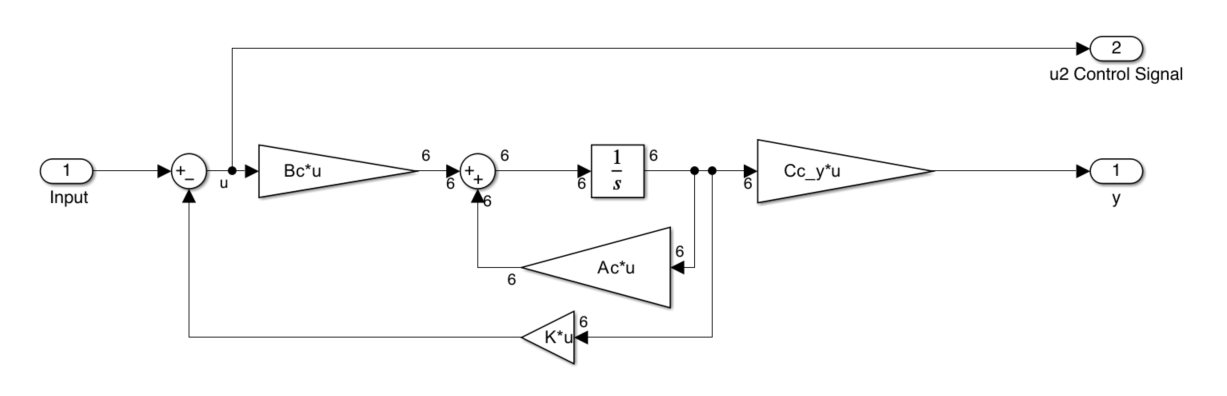
\includegraphics[scale=0.35]{State-FeedbackBlockDiagram.png}}
\caption{State-Feedback Controller Block Diagram}
\label{figure}
\end{figure}

\begin{figure}[htbp]
\centering
\centerline{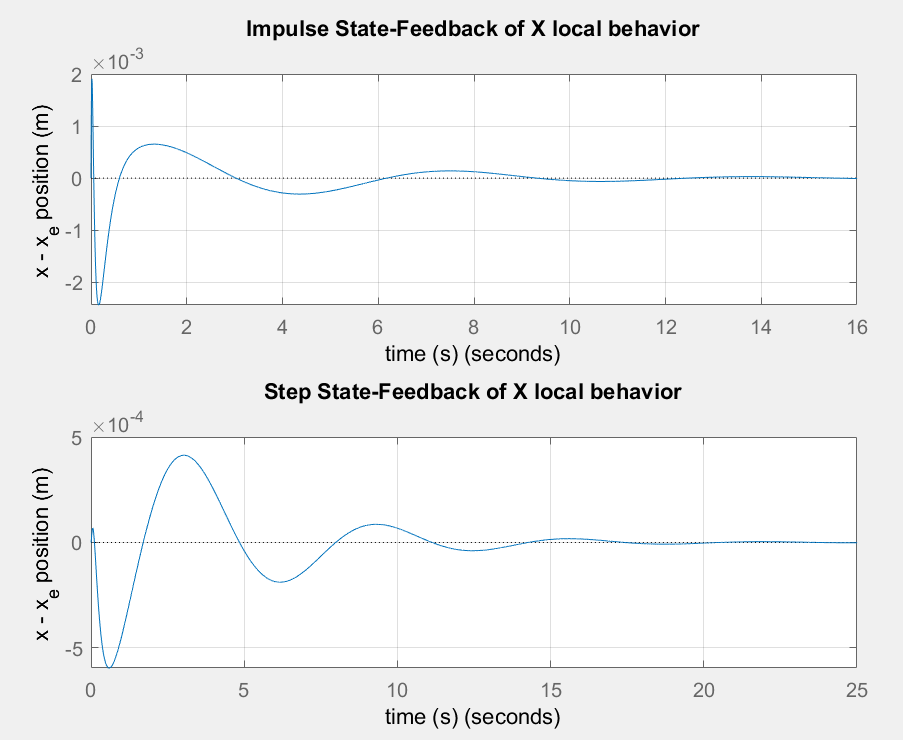
\includegraphics[scale=0.45]{X_StateFeed_StepImp.PNG}}
\caption{Impulse \& Step Local X State-Feedback Response}
\label{figure}
\end{figure}
\begin{figure}[htbp]
\centering
\centerline{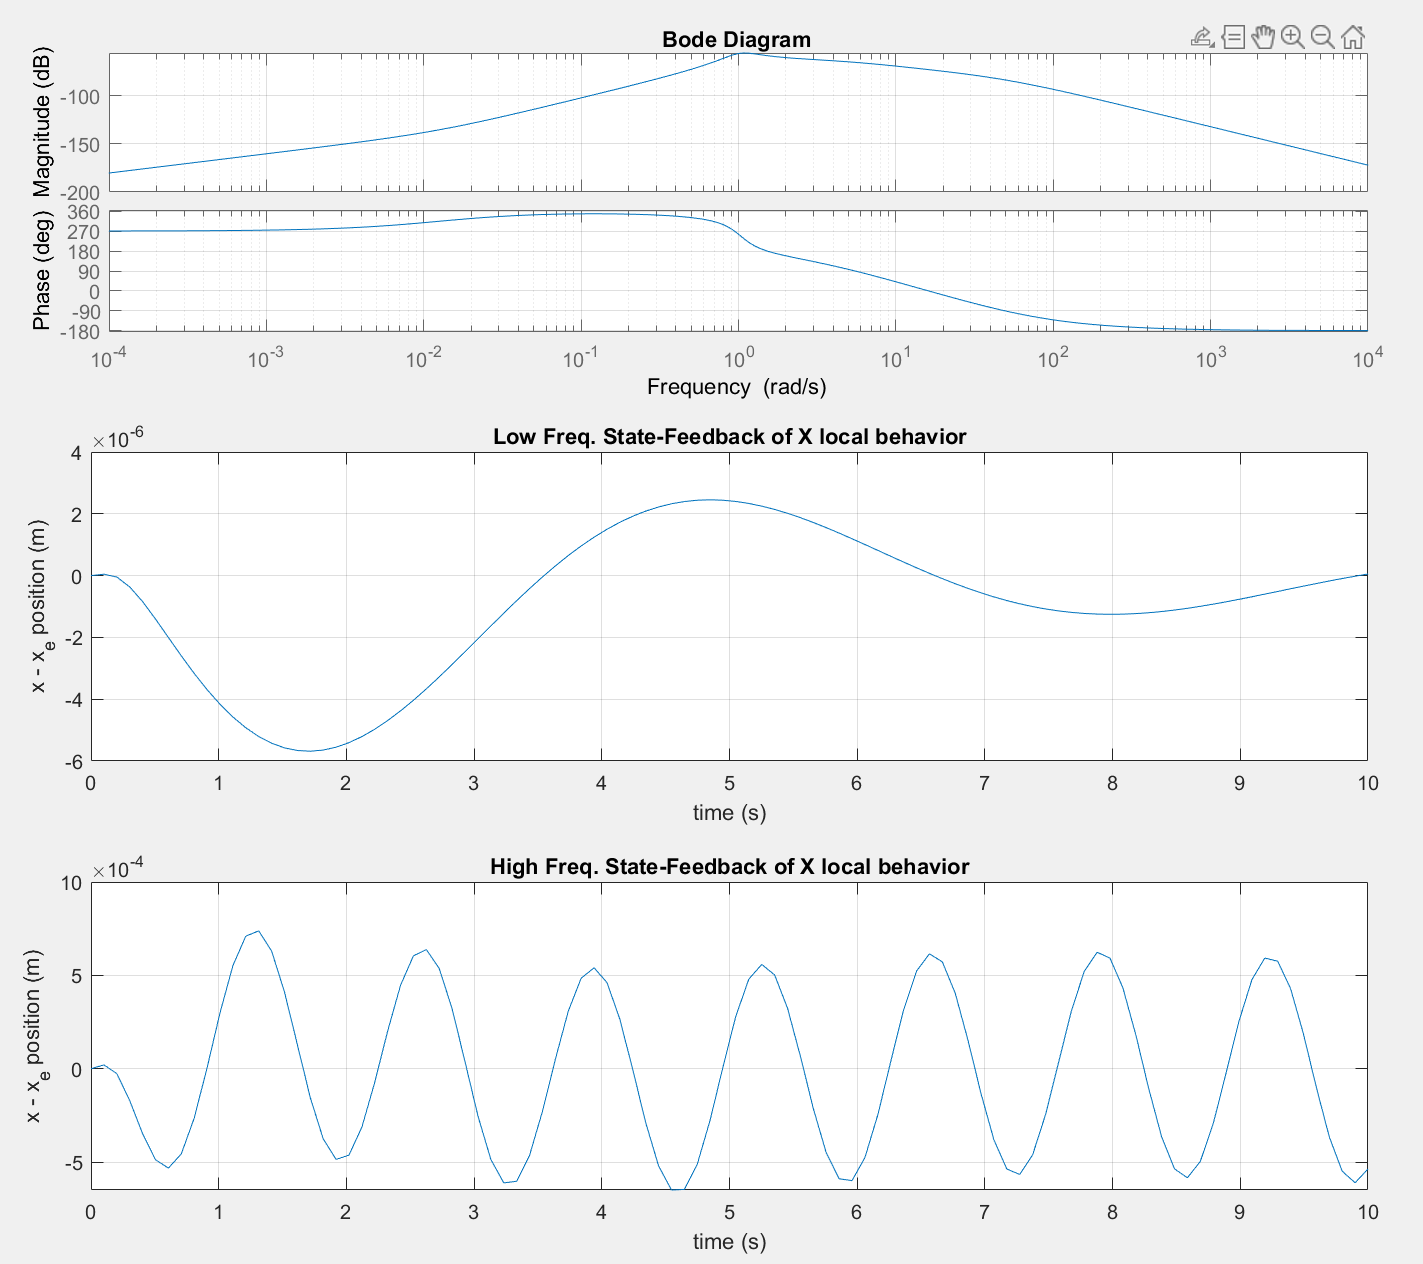
\includegraphics[scale=0.3]{X_StateFeed_Sine.PNG}}
\caption{High \& Low Freq. X State-Feedback Response}
\label{figure}
\vspace{-5mm}
\end{figure}
\begin{figure}[htbp]
\centering
\centerline{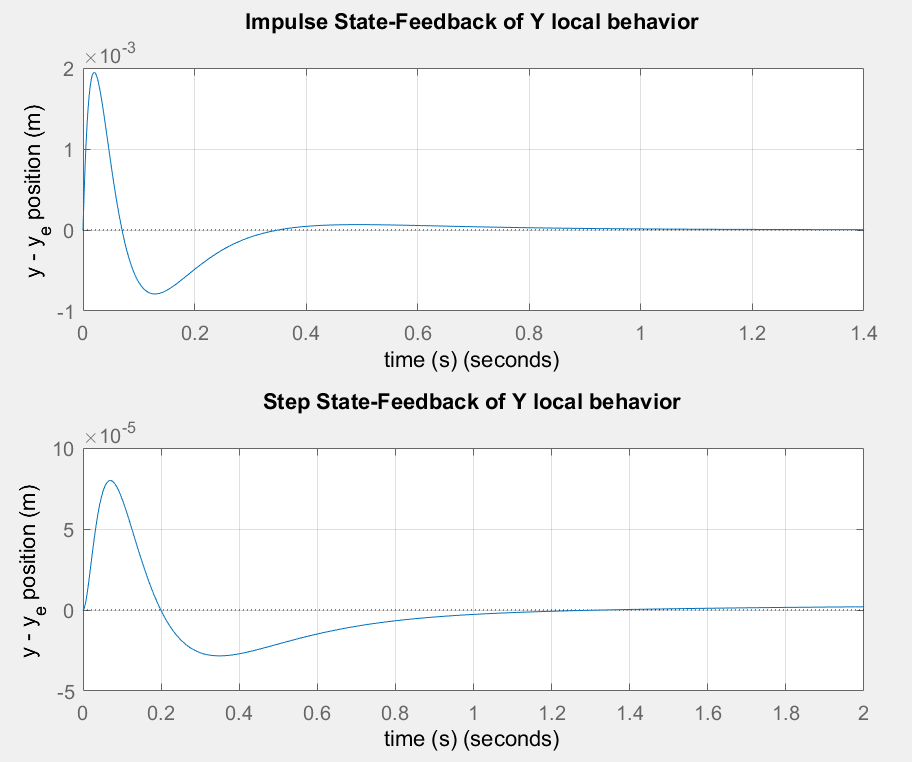
\includegraphics[scale=0.4]{Y_StateFeed_StepImp.PNG}}
\caption{Impulse \& Step Local Y State-Feedback Response}
\label{figure}

\end{figure}

\begin{figure}[htbp]

\centering
\centerline{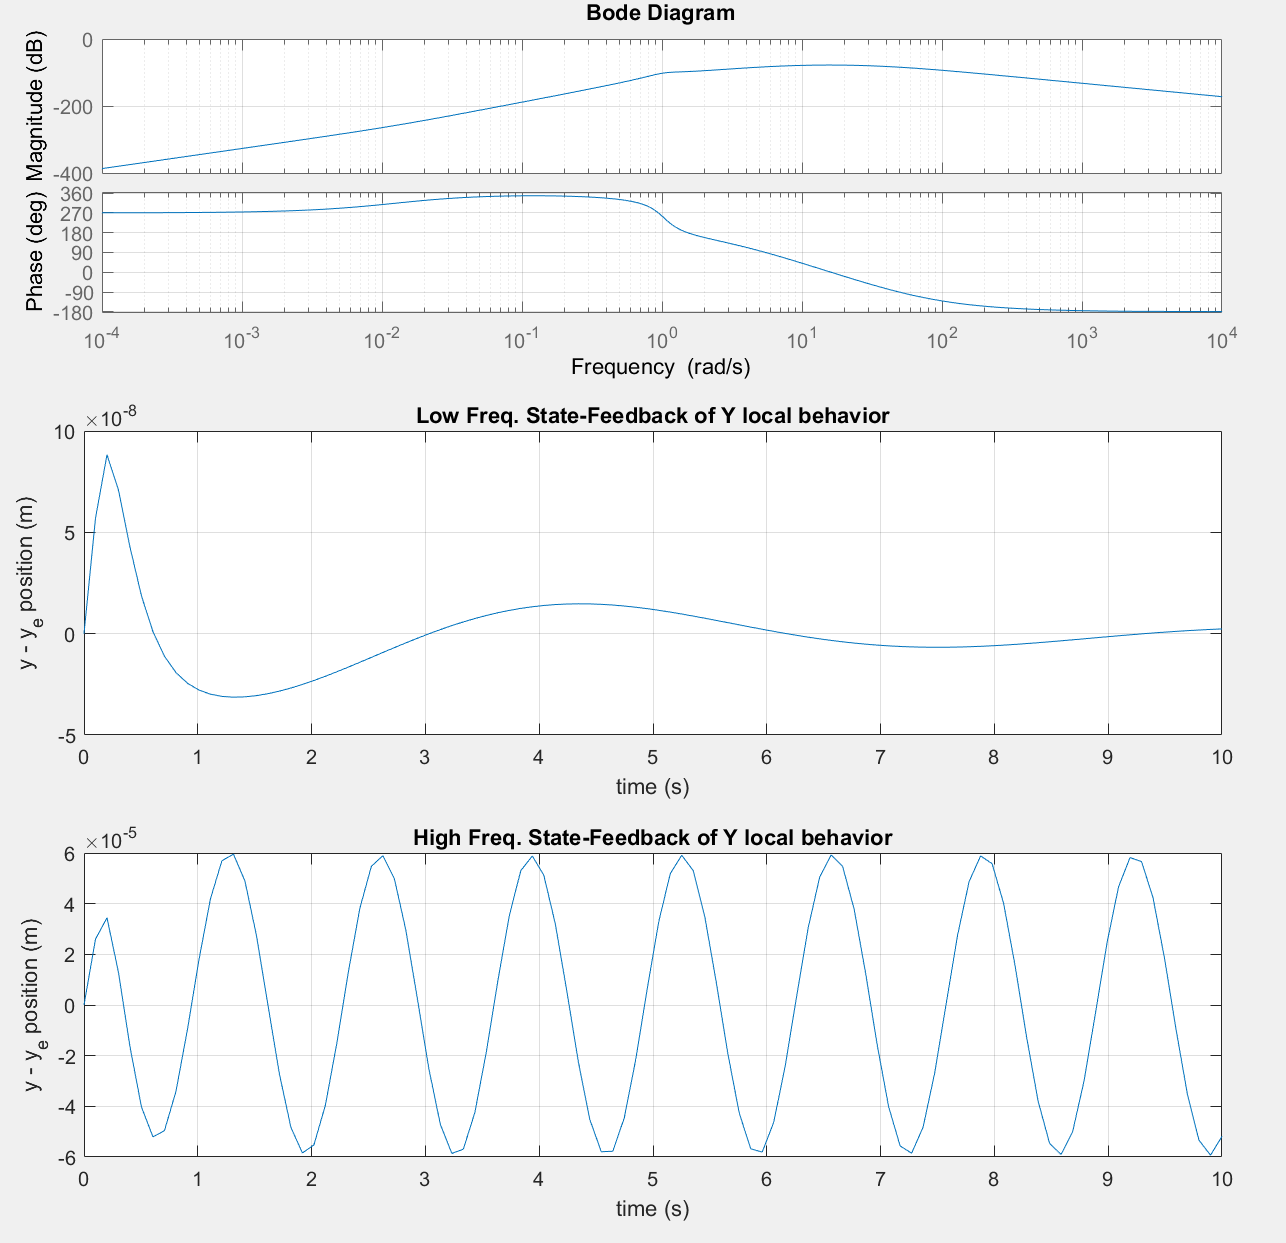
\includegraphics[scale=0.25]{Y_StateFeed_Sine.PNG}}
\caption{High \& Low Freq. Y State-Feedback Response}
\label{figure}
\end{figure}
\newpage
For the impulse/step inputs, both local x and y converge to the origin. The local x response converges later than local y because the controller is resisting the input and angular rotation ($\theta$). For high \& low frequencies, local x and y converge to an equilibrium mean. This system was stable even though the model neglected torque air resistance.  

\subsection{Observer State-Feedback Controller}
The Observer State-Feedback Controller (Equations 60-62) adds a Luenberger observer with its observer gain, $L$, (Equation 63), and a new State-Feedback Gain, $K_{obs}$,(Equation 64) to the Jacobian Matrices. These matrices are controllable and observable. Note that the Controllable Canonical Form is only controllable, and the Observable Canonical Form is only observable. The following are the desired closed-loop Observer Eigenvalues/poles:\\
$\lambda_{obs}$ = [-300 + 10j, -300 - 10j, -1500, -2000, -3000, -5000]\\
These observer eigenvalues are 5x faster than the farthest State-Feedback eigenvalues. The same State-Feedback poles are used from the State-Feedback controller. Similarly, the observer has dominant poles, and the real part of these eigenvalues is negative for stability. As previously mentioned, the poles are farther away from the origin for faster dynamics. Note that the poles are positioned so a physical actuator can achieve the desired system gains. Fig. 9 shows the Observer State-Feedback Controller block diagram. For the Observer State-Feedback controller, Fig. 10-11 \& Fig. 12-13 are local x and y responses respectively. Note that the observer and plant have no initial conditions, thus their responses are the same.  
\[
\zeta^\prime = A\zeta -BK_{obs}\hat{\zeta} + Bv\tag{60}
\]
\[
\hat{\zeta}^\prime = LC\zeta + (A - LC -BK_{obs})\hat{\zeta} + Bv
\tag{61}
\] 
\[
R = C\zeta + Dv
\tag{62}
\] 
\[
L =  
\begin{bmatrix}
7924   &    2920.9\\
548.02    &     4176\\
-1.3774E+09  &-2.0221E+09\\
1.7855E+07  & 1.5155E+07\\
1.2037E+06  & 3.6446E+06\\
-2.7043E+11  &-4.7547E+11\\
\end{bmatrix}
\tag{63}
\] 
\[
K_{obs} =  
\begin{bmatrix}
-8   & -31  & 86  & -13 & -3  &  10\\
 71  &  946 &-1189  & 305 &  161  & -83\\
\end{bmatrix}
\tag{64}
\] 

\begin{figure}[htbp]
\centering
\centerline{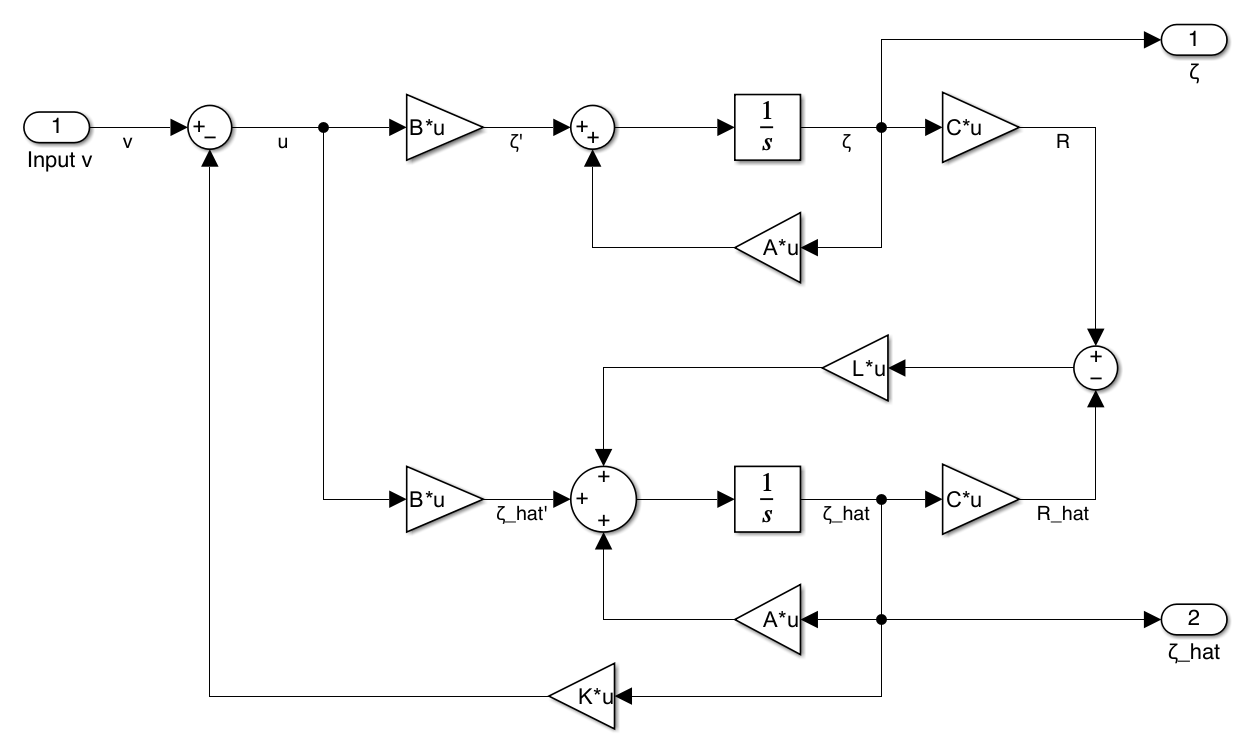
\includegraphics[scale=0.3]{ObserverStateFeedback.png}}
\caption{Observer State-Feedback Controller Block Diagram}
\label{figure}
\end{figure}

\begin{figure}[htbp]
\centering
\centerline{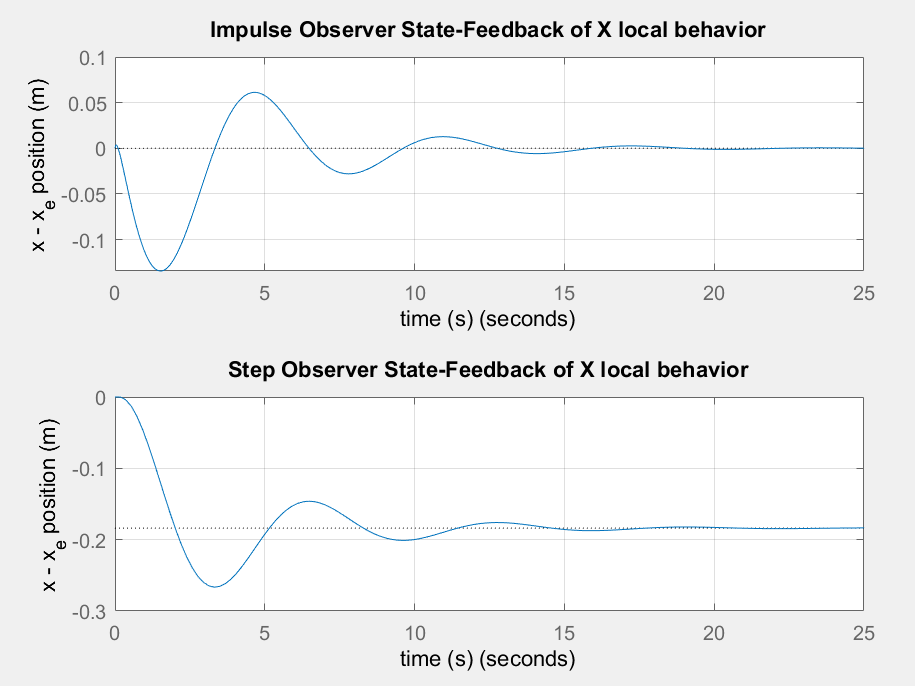
\includegraphics[scale=0.4]{X_OSF_StepImp.PNG}}
\caption{Impulse \& Step Local X Observer State-Feedback Response}
\label{figure}
\end{figure}

\begin{figure}[htbp]
\centering
\centerline{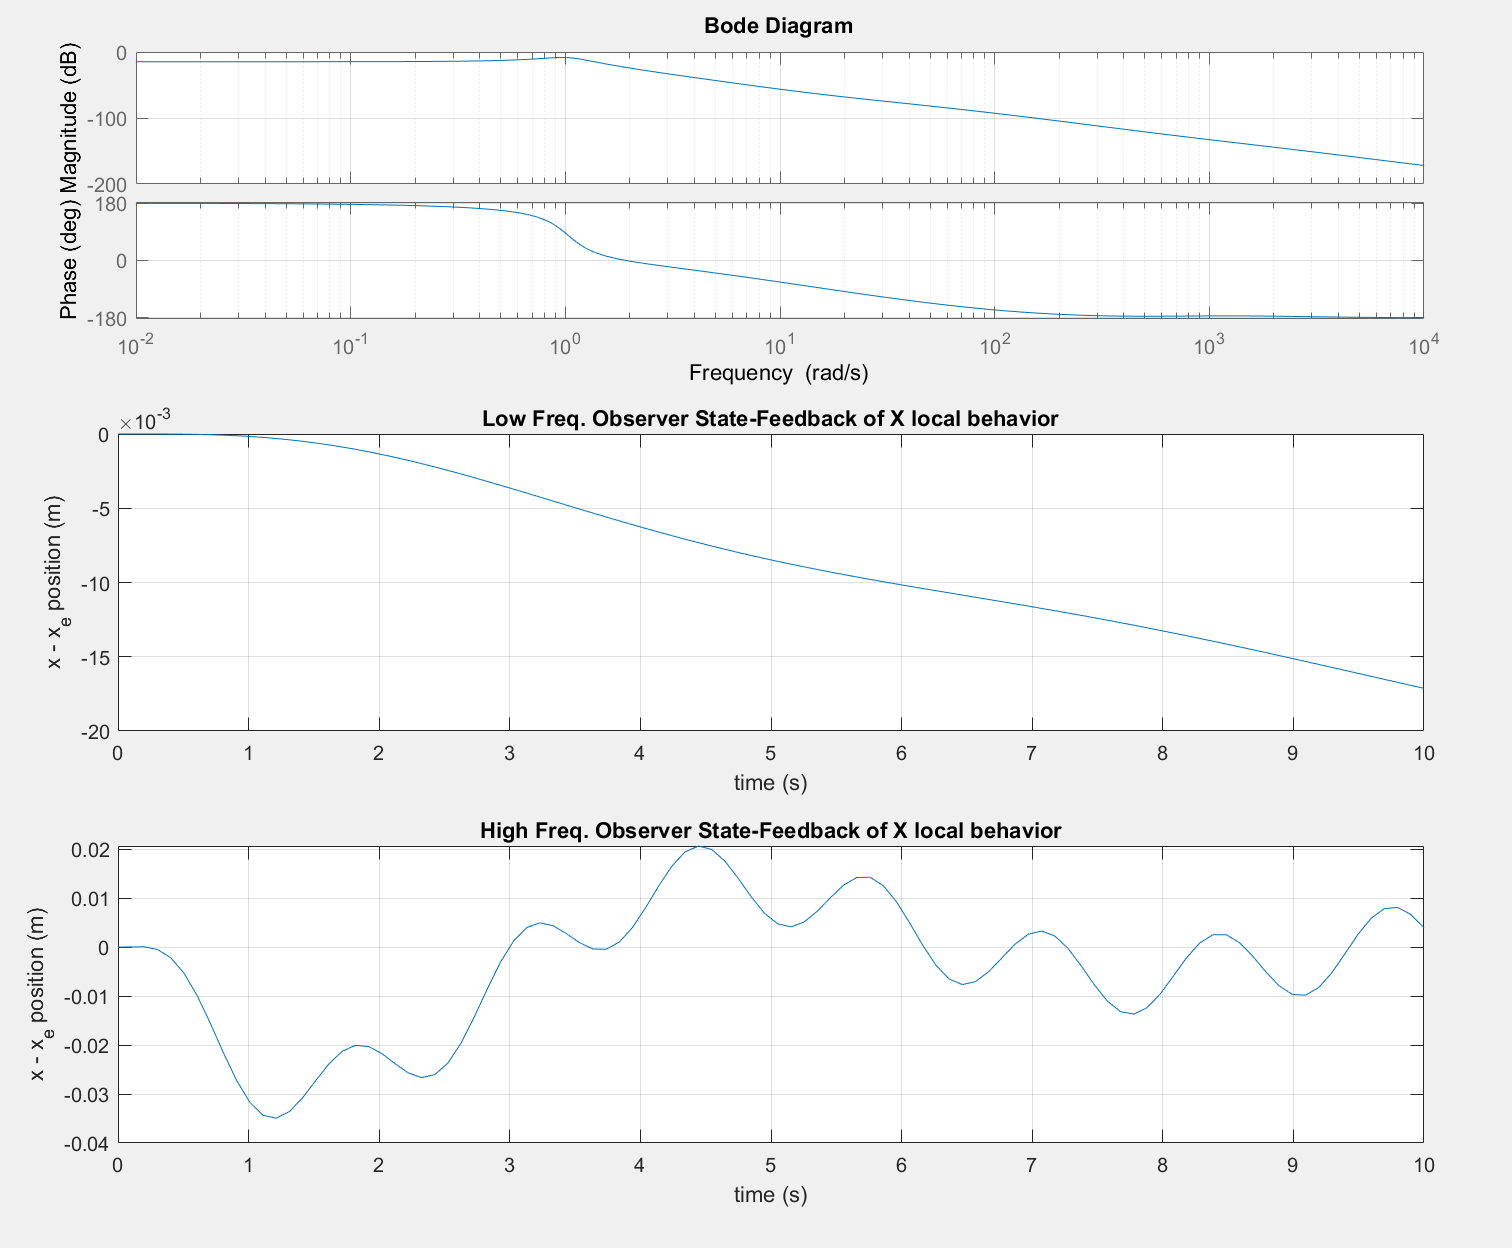
\includegraphics[scale=0.3]{X_OSF_Sine.PNG}}
\caption{High \& Low Freq. X Observer State-Feedback Response}
\label{figure}
\vspace{-5mm}
\end{figure}

\begin{figure}[htbp]
\centering
\centerline{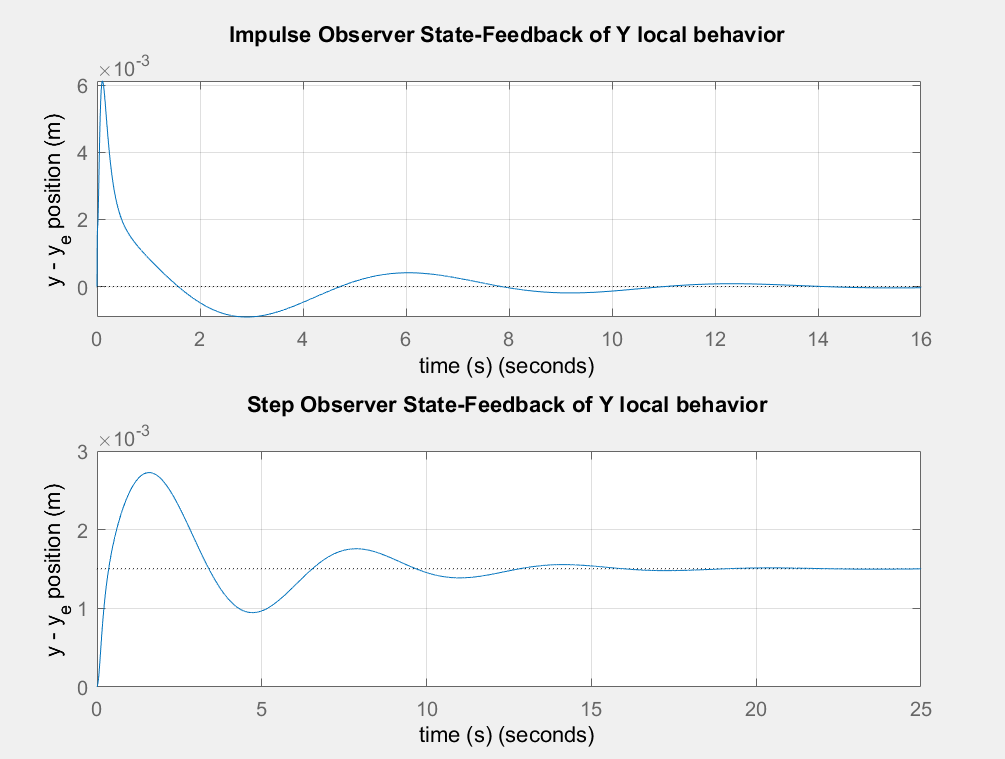
\includegraphics[scale=0.4]{Y_OSF_StepImp.PNG}}
\caption{Impulse \& Step Local Y Observer State-Feedback Response}
\label{figure}
\end{figure}

\begin{figure}[htbp]
\centering
\centerline{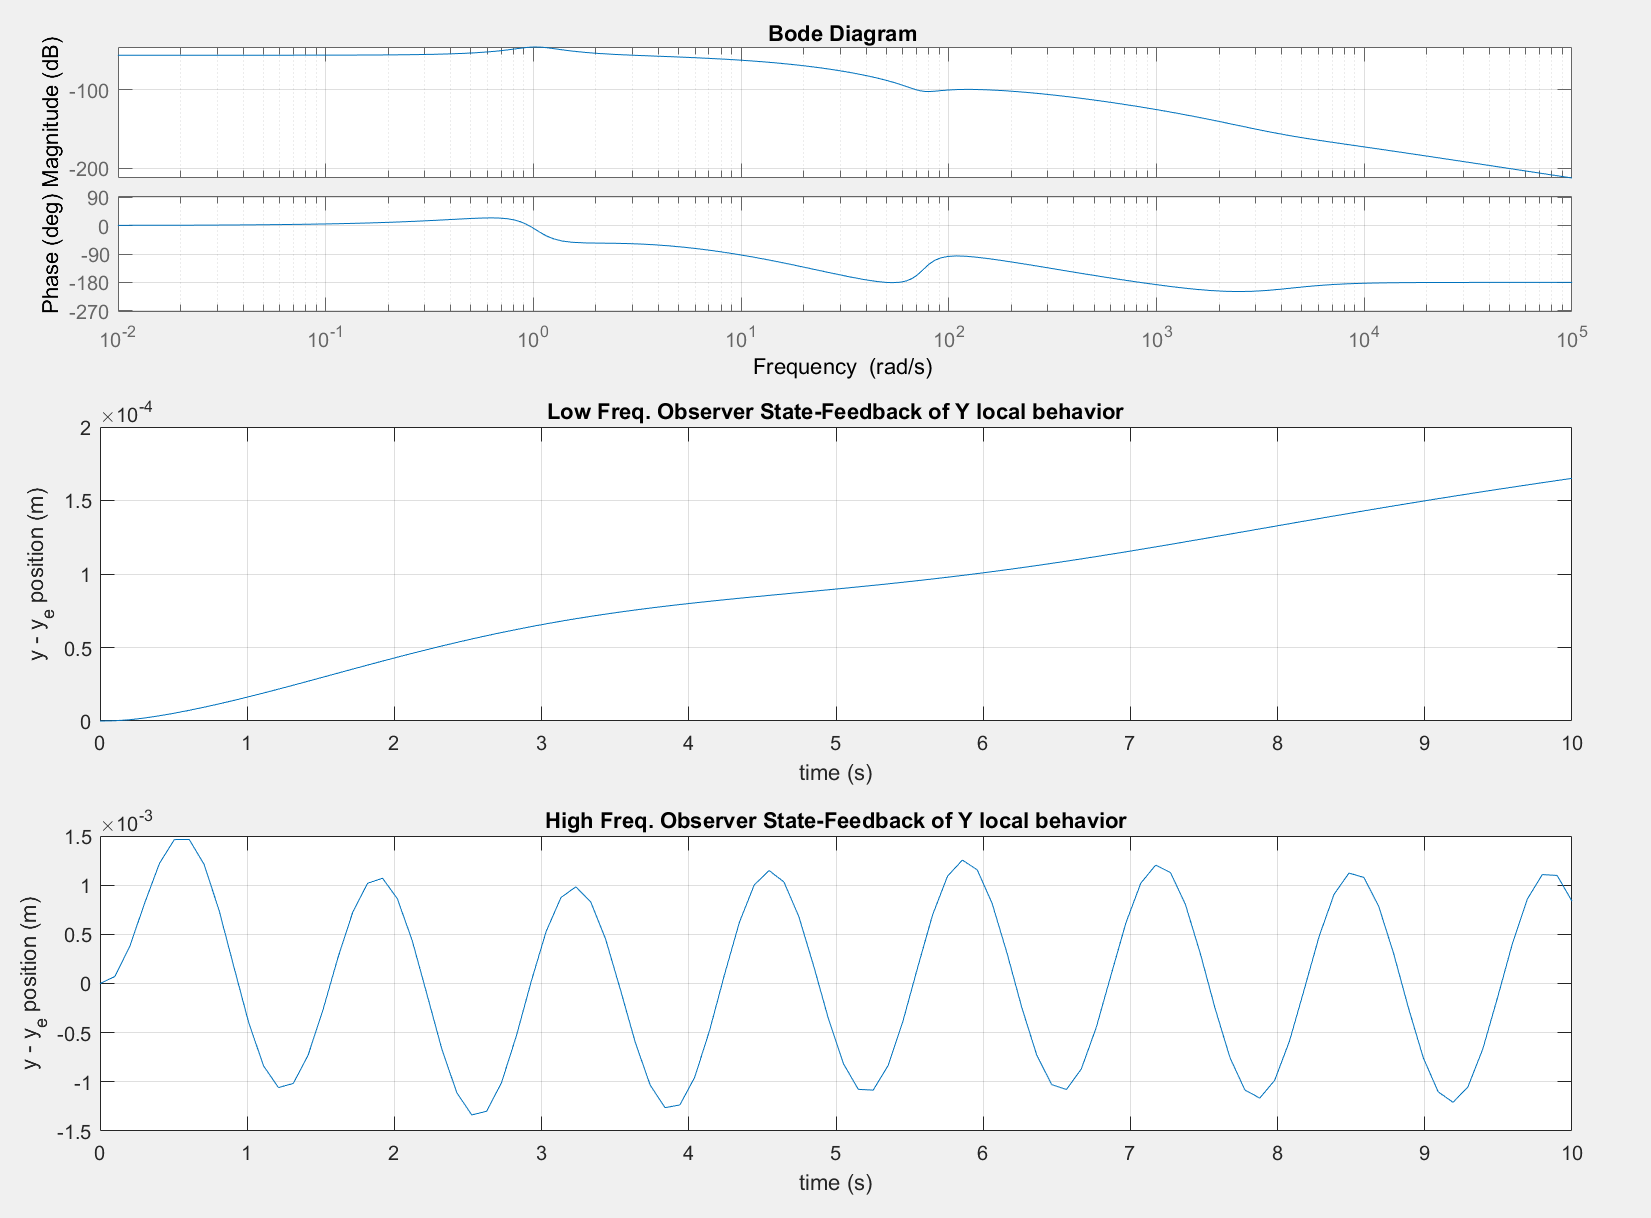
\includegraphics[scale=0.25]{Y_OSF_Sine.PNG}}
\caption{High \& Low Freq. Y Observer State-Feedback Response}
\label{figure}
\end{figure}

\newpage
Similarly, the local x and y responses reach a steady-state value for step and impulse inputs. For high \& low frequencies, the responses converge to a steady-state equilibrium mean.  These Observer State-Feedback responses are slower to converge than the State-Feedback. When the plant state variables ($\zeta$) are immeasurable, the Observer state variables ($\hat{\zeta}$) approximate the plant state variables. Note that if the Observer had different initial conditions than the plant, the responses of the Observer will approximate the aircraft's positional responses. 

\section{Conclusion}
The nonlinear 2D vectored thrust aircraft is linearized and successfully controlled by a State-Feedback and Observer State-Feedback controller for a step, impulse, \& sine inputs. This aircraft was stable even though the model neglected torque air resistance.  For future applications, nonlinear State-Feedback and Observer controllers can be implemented to control the original nonlinear system (Equations 1-3). The model can include vertical takeoff and landing maneuvers and external disturbances inputs. \\

\section{Group Contribution Breakdown}
Reese: Physics Derivation, FBD, Nonlinear, and Linear MATLAB/Simulink Models, Block Diagrams, Interpretation/analysis of linear/nonlinear results, State Feedback, and Observer State-Feedback design.\\

Sayed: Nonlinear Simulink Model, Linearizing Nonlinear System, Analysis, Mathematical Reviewer, and Stability Analysis/Interpretations.  \\

Tyler: Problem Formation, Linearizing Nonlinear System \& calculating Analytical/Numerical stability, state-space representations, \& transfer functions. Simulating State-Feedback \& Observer State-Feedback Controllers. Create an Overleaf template with Model/Physics description, Model equations, Analytical \& Numerical Analysis, Controller Simulations, References, and MATLAB Results. \\

\section{References}
\noindent [1] K. J. Åström, R. M. Murray, \textit{Feedback Systems: An Introduction for Scientists and Engineers.} Princeton University Press, 2008. [Online]. Available: http://www.cds.caltech.edu/$\sim$murray/books/AM08/pdf/fbs-public\_24Jul2020.pdf. 
Accessed: Feb. 10, 2024. \\

\noindent [2] C. S. Huang and K. Yuan.
“Output Tracking of a Non-Linear Non-Minimum Phase PVTOL Aircraft Based on Non-Linear State Feedback Control”, International Journal of Control, vol. 75, no. 6, pp. 466–473, 2002. Accessed on: March 7, 2024. [Online]. Available: doi:10.1080/00207170210121907.\\

\end{document}